\documentclass[a4paper]{article}
%\usepackage{simplemargins}

%\usepackage[square]{natbib}
\usepackage{hyperref}
\usepackage{array}
\usepackage{amsmath}
\usepackage{amsfonts}
\usepackage{amssymb}
\usepackage{graphicx}
\usepackage[a4paper]{geometry}
\usepackage{indentfirst}
\newcommand\tab[1][1cm]{\hspace*{#1}}
\graphicspath{{images/}}
\geometry{
    left=20mm,
    top=20mm,
}
\hypersetup{
    colorlinks=true,
    linkcolor=blue,
    urlcolor=blue,
    pdftitle={Overleaf Example},
    pdfpagemode=FullScreen,
}
\urlstyle{same}

\begin{document}
\pagenumbering{gobble}

\Large
 \begin{center}
    \textbf{Software Requirement Specification\\
        Linear Programing Case Solver (Lipcas)
        V 0.1.1
    }

\hspace{10pt}

% Author names and affiliations
\large
M. Rizqi R$^1$, Anggun Kurniatul Hidayah$^2$,
Abdul Rahman $^3$ \\

\hspace{10pt}

\small  
$^1$) First affiliation\\
20051204034\\
$^2$) Second affiliation\\
20051204006\\
$^3$) Third affiliation\\
20051204052

\date{today}

\end{center}

\hspace{10pt}

\normalsize
\section*{1. Pendahuluan}
    \subsection*{1.1 Tujuan Penulisan Dokumen}
    \noindent Dokumen ini ditulis untuk memberikan penjelasan rinci
    tentang spesifikasi program kalukator yang dibuat.
    Aplikasi ini dibuat dalam rangka memenuhi permintaan
    Universitas Negeri Surabaya untuk membuat sebuah aplikasi 
    yang bisa digunakan untuk memecahkan masalah pada bidang 
    pemrograman linear, seperti fungsi, pertidaksamaan,
    grafik, dan juga uji titik dari input yang dimasukkan
    oleh pengguna.
    \subsection*{1.2 Ruang Lingkup}
    \noindent 
    \begin{enumerate}
        \item Software bisa diakses secara \textit{offline}.
        \item Aplikasi berbasis \textit{desktop}.
        \item Terdapat dua jenis pengakses yaitu admin dan user.
        \item Penyelesaian model kasus berupa fungsi, pertidaksamaan, grafik dan uji titik.
        \item Aplikasi dapat berjalan di segala jenis sistem operasi dengan syarat memiliki Python Intrepeter
    \end{enumerate}
    \subsection*{1.3 Batasan Masalah}
    \begin{enumerate}
        \item Aplikasi hanya bisa menampilkan output berupa \textit{text-based}.
        \item Aplikasi hanya berupa CLI (\textit{Command Line Interface}).
    \end{enumerate}
    \subsection*{1.4 Nama Software}
    \noindent \textit{Linear Programming Case Solver} (Lipcas)
    \subsection*{1.5 Definisi }
    \begin{tabular}{ | m{1em}| m{0.2\textwidth} | m{0.7\textwidth} | }
        \hline
        \textbf{No.} & \textbf{Istilah} & \textbf{Definisi}\\
        \hline
        1 & Software & Merupakan Bahasa Inggris dari perangkat lunak.\\
        \hline
        2 & Offline & Merupakan Bahasa Inggris dari "Luring" yang berarti tidak
        membutuhkan jaringan internet dalam penggunaannya.\\
        \hline
        3 & Sistem Operasi & Sebuah perangkat lunak yang dibutuhkan
        agar pengguna bisa menggunakan sebuah PC/Laptop/ perangkat lain
        yang serupa fungsinya dengan komputer.\\
        \hline
        4 & Admin & Jenis pengguna yang memiliki akses penuh terhadap
        semua data yang tersimpan.\\
        \hline
        5 & User & Jenis pengguna yang memiliki akses terbatas terhadap
        data dan kelakuan aplikasi.\\
        \hline
        6 & Database & Tempat dimana semua data tersimpan dan dapat dikelola
        oleh program.\\
        \hline
        7 & Output & Merupakan hasil keluaran dari suatu perintah saat program
        selesai atau sedang dijalankan\\
        \hline
        8 & Input & Merupakan masukan yang diberikan oleh pengguna dengan tujuan 
        agar program dapat memproses masukan tersebut.\\
        \hline
        9 & Command Line Interface & Adalah antar muka berbasis teks tanpa gambar.\\
        \hline
        10 & Python & Bahasa pemrograman yang digunakan pada perangkat lunak \\
        \hline
    \end{tabular}

    \subsection*{1.6 Kepanjangan}
    \begin{tabular}{ | m{1em}| m{0.2\textwidth} | m{0.7\textwidth} | }
        \hline
        \textbf{No.} & \textbf{Singkatan}   & \textbf{Kepanjangan}\\
        \hline
        1 & SRS & \textit{Software Requirement Specification}\\
        \hline
        2 & RAM & \textit{Random Access Interface}\\
        \hline
        3 & CPU & \textit{Central Processoring Unit}\\
        \hline
        4 & GB & \textit{Gigabyte}\\
        \hline
        5 & MB & \textit{Megabyte}\\
        \hline
        6 & MHz & \textit{Megahertz}\\
        \hline
        7 & UNESA & Universitas Negeri Surabaya \\
        \hline
    \end{tabular}
    \subsection*{1.7 Referensi}
    \noindent Berikut referensi yang digunakan untuk pengembangan perangkat
    lunak Lipcas:

    \vspace*{10pt}
    \begin{tabular}{ | m{1em}| m{0.8\textwidth} | }
       \hline 
       \textbf{No} & \textbf{Referensi}\\
       \hline
       1 & \href{https://wiki.python.org/moin/BeginnersGuide}{Dokumentasi Python} \\
       \hline
       2 & \href{https://docs.python.org/3/library/tk.html}{Python Tkinter Library}\\
       \hline
    \end{tabular}

    \subsection*{1.8 Penjelasan Umum}
    \noindent Aplikasi dapat menampilkan informasi menu mengenai
    pembuatan fungsi, pertidaksamaan, grafik, dan titik uji
    dari suatu permasalahan matematis. Setelah itu pengguna 
    dapat melihat hasil kalukasi dari masukan yang telah diberikan
    sesuai menu yang dipilih. Data keluaran akan disimpan dalam
    \textit{database} yang bisa diakses melalui menu "Riwayat".

\section*{2. Gambaran Umum}
    \subsection*{2.1 Karakteristik Pengguna}
    \begin{enumerate}
        \item Pengguna harus bisa menggunakan satu dari 4 sistem operasi yang ada (Windows, GNU/Linux, *BSD, MacOS).
        \item Pengguna merupakan \textit{User/Admin} yang terdaftar.
        \item Pengguna mengerti tentang \textit{Linear Programming}.
        \item Pengguna memahami cara kerja program.
    \end{enumerate}
    \subsection*{2.2 Jenis Pengguna}
    \begin{enumerate}
        \item User 
        \item Admin
    \end{enumerate}
    \subsection*{2.3 Hak Akses Pengguna}
    \begin{enumerate}
        \item User : Bisa mengoperasikan \textit{Linear Programming}.
        \item Admin : Bisa melakukan segala bentuk manipulasi program, terutama manipulasi data dan jenis operasi.
    \end{enumerate}
    \subsection*{2.4 Ketergantungan Software}
    \noindent Program ini dibuat seminimal mungkin sehingga tidak membutuhkan
    sumber daya yang besar ketika menjalankannya. Hanya dengan sebuah sistem operasi
    yang telah terpasang Python Intrepeter beserta \textit{library} yang 
    dibutuhkan, maka program dapat berjalan dengan semestinya.
    \subsection*{2.5 Spesifikasi Pendukung Software}
    \begin{enumerate}
        \item Satu dari 4 sistem operasi (Windows, GNU/Linux, *BSD, MacOS).
        \item Python Intrepeter
        \item Python Library yang dibutuhkan
        \item Minimal 512MB Free RAM 
        \item Minimal 1 Physical Core CPU
        \item Minimal 4MB CPU cache
        \item 200MB storage
    \end{enumerate}
\section*{3. Analisis Kebutuhan}
    \subsection*{3.1 Identifikasi Aktor}
    \begin{enumerate}
        \item Mahasiswa UNESA sebagai pengguna aplikasi yang
        membutuhkan kalkulasi permodelan \textit{Linear Programming}.
        \item Admin yang berhak untuk memantau keadaan sistem 
        dan melakukan manipulasi pada data.
    \end{enumerate}
    \subsection*{3.2 Identifikasi Use Case}
    \begin{enumerate}
        \item Melakukan login untuk masuk kedalam sistem
        \item Pengelolaan data informasi dalam dashboard
        seperti manipulasi akun user dilakukan oleh admin.
        \item Permodelan kasus untuk membuat fungsi, pertidaksamaan,
        grafik, dan uji titik.
        \item Riwayat kasus diakses untuk memudahkan pengguna melihat
        kembali perhitungan yang telah dilakukan tanpa mengulang
        perhitungan tersebut dari awal.
    \end{enumerate}
    \subsection*{3.3 Diagram Use Case}
    \begin{center}
    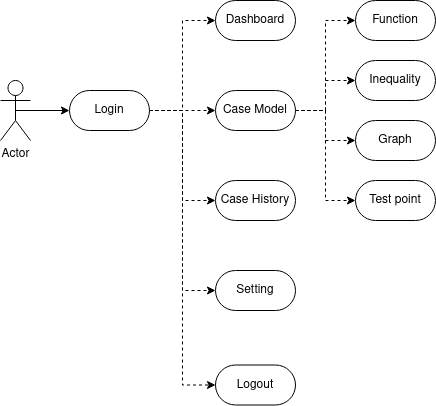
\includegraphics[width=0.5\textwidth]{uml-Use Case.drawio.png}
    \end{center}
\section*{4 Skenario}
    \subsection*{4.1 Use Case Login}

\end{document}
